\section{Introduction}
The $x2x$ network makes use of a decentralized and privacy-oriented digital currency that evolves the CryptoNote protocol\cite{CryptoNote} through the groundbreaking discoveries in the field of Byzantine consensus and pseudo-random functions of world renown cryptographers such as Silvio Micali, Michael Rabin, Alexander Yampolskiy and Evgeniy Dodis. $x2x$ radically departs from any other blockchain by employing an adaptive consensus mechanism, called Segregated Byzantine Agreement (or SBA{$\large\star$}), which does not require the computational intensity of proof-of-work and is a fairer alternative to proof-of-stake. Built on such consensus algorithm, $x2x$ is poised to be the first to simultaneously achieve previously conflicting goals of guaranteeing transaction untraceability and unlinkability, safeguarding user privacy, reaching transactional "finality" after a bound number of rounds within a single block election and achieving virtually unbounded user scalability without any significant performance degradation.

The $x2x$ network requires a heightened security setup designed specifically to:

\begin{enumerate}
\item Obfuscate IP addresses of the communicating peers
\item Prevent linkability and traceability of accounts
\item Guarantee network performance
\item Implement efficient payment mechanism for high QoS applications such as secure and anonymous voice calls
\end{enumerate}

An important difference with CryptoNote, is that $x2x$ does not make use of proof-of-work mining and therefore drops completely CryptoNight and deviates substantially from the hashing algorithms therein adopted. In particular, $x2x$ uses what we call \hyperref[sec:SBA]{Segregated Byzantine Agreement} (SBA$\large\star$) protocol which enhances classic BA$\large\star$ by implementing specific measures to protect peer privacy. SBA$\large\star$ has been developed specifically to power the $x2x$ Blockchain and help meeting the aforementioned requirements. These efforts do not solely relate to the application layer but extends to the networking layer as well. This is why the $x2x$ protocol makes use of:

\begin{itemize}
\item \textbf{Stealth addresses}: to protect transaction recipient anonymity
\item \textbf{RingCT signature}: to protect transaction sender's identity
\item \textbf{Anonymous Network Layer}: to protect the IP address of the network peers; to provide secure data transfer mechanism; to implement off-line data retrieval strategy; to power the anonymous gossip network for transaction propagation and verification
\item \textbf{Non-Interactive Verifiable Secret Sharing Scheme}: to conceal all but highest priority time-locked transactions from the participants to the Block Generation sortition
\item \textbf{Cryptographically Committed Provisioners}: to protect the information about stake; to implement a division of responsibilities between Block Generators and the electable Block Voters and Verifiers; to boost network efficiency by acting as state channel guarantors; to incentivise participation to the network; to protect the balance information of transacting nodes; to prepare SBA$\large\star$ for future expansion with non-balance and non-payment related weights such as storage contributed to the network (as in proof-of-storage), availability expressed in elapsed time since joining the network (as in proof-of-idle), etc.
\end{itemize}

\section {Preliminaries}

\subsection{Diffie-Hellman Hardness Assumption}

In any group, a discrete logarithm $log_b\space$ a is a number x $\in \mathbb{Z}$ such that $b^x = a$. 

Most of the cryptographic building blocks related to this work are linked to the Diffie-Hellman assumption which uses the hardness of discrete logarithms in cyclic groups \cite{CyclicGroup}. Considering a multiplicative cyclic group $\mathbb{G}$ of order $p$ and generator \cite{Generator} $g$, we can formulate the following assumption: given $g^a$ and $g^b$ for uniformly and independently chosen $a$ ,$b$ $\in \mathbb{Z}_p$ then $g^{ab}$ performs like a random element in $\mathbb{G}$ of order $p$.

As a consequence of such assumed randomness, the Decisional Diffie-Hellman (DDH) Problem relates to distinguishing the following two probability distributions:

\begin{itemize}
\item ($g^a, g^b, g^{ab}$) $\forall \space a,b \in \mathbb{Z}\\$ // $\small (g^a, g^b, g^{ab}) \textrm{ are defined as a Diffie-Hellman Tuple}$
\item ($g^a, g^b, g^{c}$) $\forall \space a,b,c \in \mathbb{Z}$
\end{itemize}

\subsection{Hiding Recipients: Stealth Addresses}
Inspired by the CryptoNote white-paper\cite{CryptoNote}, stealth address technology is at the basis of $x2x$ recipient hiding technique. Already widely tested in other privacy-oriented digital currencies, it is the proven choice for concealing the true recipient address of a transaction while keeping uniqueness within the context of the ledger (meaning no other address can be linked to a stealth address). Additionally, a derivation of an unbound number of receiving addresses is also possible without any of them allowing traceability back to the recipient's main address. As an anonymous key agreement protocol, $x2x$ uses the Elliptic Curve Diffie-Hellman (ECDH) due to the desired property of allowing two parties to generate a shared secret by solely knowing each other's public key, and the generator point of the Elliptic Curve used in the Twisted Edward equation. Following is a detailed explanation of how $x2x$ implements Stealth Address technology. 

\subsubsection{Elliptic-Curve Cryptography}

The system makes use of Elliptic-Curve Cryptography (ECC), hence approaching public-key cryptography through the algebraic structure of elliptic curves and thus allowing for the creation of smaller and more efficient cryptographic keys. ECC gives the same security levels of, for example, RSA, but using a much smaller security key.

The structure of an elliptic curve is a plane curve satisfying the equation $y^2=x^3+ax+b$, which returns us the graph in Figure \ref{fig:elliptic}.

\begin{figure}
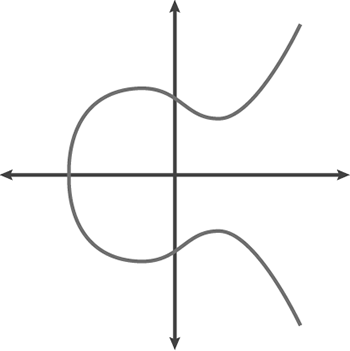
\includegraphics[height=1in, width=1in]{elliptic_bn}
\caption{A generic elliptic curve}
\label{fig:elliptic}
\end{figure}

In ECC, a Galois Field is created by taking the modulo of all points using a large prime number, creating a finite number of values for the used equation. The following axioms are furthermore taken into account:

\begin{enumerate}
\item A point can't be multiplied or divided by another point.
\item Any point on the curve can be added or subtracted to another point (or itself).
\item Adding a point to itself allows for scalar multiplication.
\end{enumerate}

\subsubsection{Private and Public Keys}

The $x2x$ Blockchain utilizes an \textit{Ed25519} curve, which is a Twisted Edwards curve with the following Elliptic Curve Parameters:

$q$ : a prime number; $q=2^{255}-19$ ; \textit{This is the number of points in the curve.}

$d$ : an element of $\mathbb{F}_q$; $d=-121665/121666$; \textit{Value used in the curve equation below}

$E$ : an elliptic curve equation; $-x^2+y^2=1+dx^2y^2$; \textit{The Twisted Edwards curve/equation we are using}

$G$ : a base point; $G=(x, -4/5)$; \textit{The}\textbf{**generator**} \textit{point. This is a base - starting point used for all Elliptic modulo operations.}

$l$ : a prime order of the base point; \\\space\space\space\space$l=2^{252}+27742317777372353535851937790883648493$ ;\\ \textit{The order of the base point} $G$\textit{. This defines the maximum size of scalars and the maximum number of points that can be used.}

$\mathcal{H}_s$: a cryptographic hash function $\{0,1\}^*\rightarrow\mathbb{F}_q$;

$\mathcal{H}_p$: a deterministic hash function $E(\mathbb{F}_q)\rightarrow E(\mathbb{F}_q)$;

All private and public keys in $x2x$ will be using 64 hex characters.

\subsubsection{Accounts and Addresses}

The following procedure will be used to create an address.

\begin{enumerate}
\item  We pick a random /textit{private spend key}, by generating 256 random bits, and reducing$\mod l$. We call this $b$.
\item  Rather than using \textit{Keccak\_256} (as in the CryptoNote paper), $b$ is hashed with hashing algorythm $H$(\textit{Skein\_256}). Skein has been chosen because the cost in terms of Cycles per Byte does not increase as we work on bigger message digest and it is also the fastest for long messages. We interpret the result of the hashing as an integer, reduce it $\mod l$ as before. We call this key $a$.  
\item  We generate our public spend and view keys $B=bG$ and $A=aG$
\item  We hash (network prefix (0xEF) + $B$ + $A$) with $H$.
\item  Append the first 4 bytes of this operation to (prefix + $B$ + $A$), obtaining a 69 bytes value (1 + 32 + 32 + 4)
\item  Convert this to \textit{cnBase58}.
\end{enumerate}

We will explain how stealth addresses work by first going trough a brief explanation about key exchanges on an ECC scenario, in the next section.

\subsubsection{The Elliptic Curve Diffie-Hellman}

The Elliptic Curve Diffie-Hellman (ECDH) is an anonymous key agreement protocol, a variant of the Diffie-Hellman protocol adapted to work with Elliptic-Curve Cryptography.

Thanks to ECDH, two parties can generate a shared secret over an unsecuredc connection only by knowing each other's public keys, and the generator point of the Elliptic Curve used in the ECC equation.

To demonstrate this, we will use Alice (with private key a and public key A=aG) and Bob (with private key b and public key B=bG). (Where G is the generator point)

As previously stated, points on a curve can be added together, and Alice could calculate a point C = A + B, but this could also be potentially done by anyone eavesdropping the conversation, since A and B are publicly available.

Now, let's remember that A and B are points on the elliptical curve, and that we can add a point to itself.

Alice can now calculate a new point D=aB,  and Bob can get D'=bA.

We can now prove that D=D', and thus Alice and Bob share a secret by operating on ECC and knowing each other's public keys and the generator point G:

\begin{enumerate}
\item Given a common generator point G;
\item Alice has a=5, A=5G (private and public keys)
\item Bob has b=7, B =7G
\item a · b = 35
\item Alice computes D=aB=5B=5·7G=35G
\item Bob computes D'=bA=7A=7·5G=35G
\item D=D'
\end{enumerate}

Point D has a corresponding scalar d, in the example above equal to 35, which is a shared secret between Alice and Bob

\subsubsection{Stealth Addresses}

Let's consider the diagram in Figure \ref{fig:cryptodg} from the CryptoNote whitepaper.

\begin{figure}
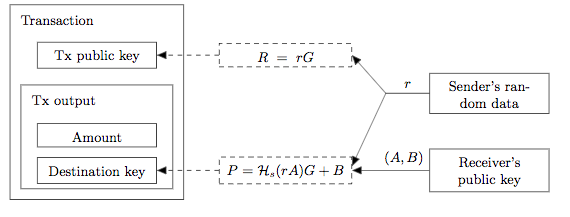
\includegraphics[height=1in]{M42G4Fy}
\caption{A \textit{stealth transaction}}
\label{fig:cryptodg}
\end{figure}

The \textit{Dual-key Stealth Address} $P$ is defined as $P=\mathcal{H}_s(rA) \cdot G+B$. The link-ability of the Stealth Address is achieved by using a combination of spend/view-keys, without actually allowing a spending transaction to take place. Let's now assume that Alice has a private \textit{spend-key} $z$ and a private \textit{view-key} $y$. We call her public \textit{spend/view-keys} $Z,Y$. On the other side, Bob's public keys are $A$ and $B$, with Bob's private keys $a$ and $b$ unknown to Alice. In order to build a stealth address, Bob needs to compute $r$ (an arbitrary random scalar chosen by Alice) and $R$ as the corresponding ECC point such as $R=rG$. $r$ is not being shared with anyone and can be discarded after its use - unless Alice wants to prove that she sent a transaction to Bob to an external party. $R$ is added to the transaction so that it can be seen by everyone. A new $r$ is calculated for each transaction, since reusing it in the computation of the Stealth Address, would result in a collision. Therefore, given the equation above: $P=\mathcal{H}_s(rA)G+B$, a Stealth Address can be constructed as follows.

\begin{enumerate}
\item P : the Stealth Address where the funds will be sent
\item $\mathcal{H}_s$ : a Hashing Algorithm returning a scalar value
\item r : the random scalar chosen by Alice
\item A : Bob's public view-key
\item G : The standard Ed25519 base point
\item B : Bob's public spend-key
\end{enumerate}

Alice calculates point D from ECDH using a randomly chosen r and Bob's public key A.

Bob computes D independently from Alice, due to the properties of ECDH.

Alice computes the scalar $f=\mathcal{H}_s(D)$ - (this hashing step creates unlinkability between Bob's address and the new stealth one) and calculates F=fG, and P = F + B (Bob's public spend-key).

Now, in order to check if he is the transaction's recipient, Bob:

\begin{enumerate}
\item Calculates D' using R as propagated with the transaction (The equality D = D'=aR is still unproven).
\item Calculates f'=$\mathcal{H}_s(D')$
\item Calculates F'=f'G
\item Calculates P'=F'+B
\end{enumerate}

If P'=P, then Bob knows the transaction was mentioned for him, and can retrieve it like this:

(Bob has to compute the secret key associated with the transaction)

\begin{enumerate}
\item Bob knows f' (computed above), and derives xf'+b  (Bob's private spend key)
\item Knowing that P=xG, we got P=xG=(f'+b)G
\item Bob then has to check if the transaction on P is spent, Bob computes a key-image and checks on the blockchain if the image linked to that transaction has been spent. Image I=x$\mathcal{H}_p(P)$
\item Bob can then sign a new transaction using x
\end{enumerate}

\subsection{Obfuscating Sender}

Ring Signatures are an efficient, established way to obfuscate the input of a transaction by making use of a sender's account keys and a number of decoy keys (called \textit{outputs}) taken directly from the blockchain, using a triangular distribution method. The technology finds its roots in the early days of blockchain research, as Satoshi Nakamoto himself was hypothesizing back in 2010:


\blockquote{Crypto may offer "key blinding". I did some research and it was obscure, but there may be something there. "Group signatures" may be related.} \footnote{https://bitcointalk.org/index.php?topic=770.msg9074\#msg9074}

The procedure allows one of the members of the \textit{ring} to sign messages on behalf of the whole group, and by doing so it renders infeasible to know exactly which member made the signing. (Figure \ref{fig:ringsig})

\begin{figure}
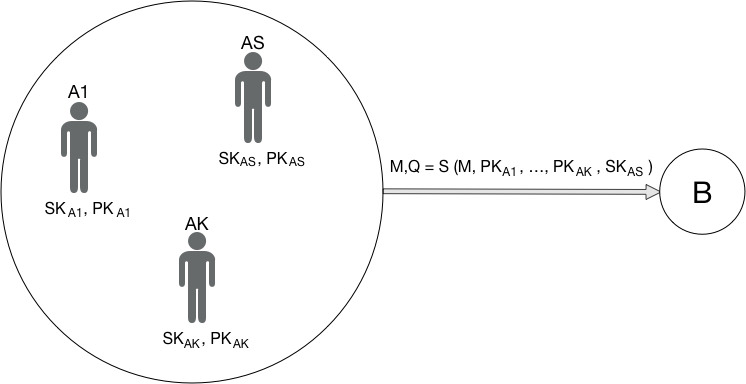
\includegraphics[scale=0.35]{ringsig}
\caption{A \textit{ring signature transaction}}
\label{fig:ringsig}
\end{figure}

In a group signature procedure, there is no central management or setup - all the signer needs is the public keys of the members she chooses to be part of the ring.

Each signer is associated with a public key $PK_x$ and a corresponding private key $SK_x$. A ring signature scheme is defined by two procedures:

\begin{itemize}
\item $\textrm{ringSign}(M, PK_1, PK_2, ..., PK_r, s, SK_s)$: which is a method for computing the ring signature Q, which gets the message M, the public keys of the ring members, and the private key of the message signer.
\item $\textrm{ringVerify}(M,Q)$: which is a procedure to verify the signature Q, which gets message M and signature Q as arguments, and returns a boolean (correct / not correct) as output.
\end{itemize}

\subsubsection{Signature Generation}

Having a message $m$ and its own private key $SK_s$, together with a sequence of ring member's public keys, signer $A_s$ can create a signature as follows:

\begin{enumerate}
\item Computes a key $k=h(m)$, where $h$ is a collision-resistant hash function.
\item Chooses a random $v$
\item Chooses a random $x_i$ and computes $y_i=g_i(x_i)$
\item Solves for $y_s$ the equation containing the \textit{Combining function} $C_{k,v}(y_1,y_2,...,y_r) = v$
\item Finds $x_s$ knowing its own $SK_s$: $x_s=g_s^{-1}$
\item Creates a ring signature: $v; x_1, x_2, ..., x_r$
\end{enumerate}

\subsubsection{Signature Verification}

A verifier can confirm a ring signature as follows, having the collection of the member's *public keys:*

\begin{enumerate}
\item Compute, for each $x_1$, $y_1=g_i(x_1)$
\item Computes $k=h(m)$
\item Confirms the equation $C_{k,v}(y_1,y_2, ..., y_r)=v$ for values of $y_i$
\item If the equation is correct then the signature is valid, otherwise it's not.
\end{enumerate}

\subsubsection{Ring Confidential Transactions}

Blockchains such as Monero use a particular breed of ring signatures called Ring Signature Confidential Transactions (\textit{RingCT}), where the privacy is taken one step further by not only giving full anonymity at the sender level (as explained above), but also on the amount spent and destination.

The RingCT technology makes the payment virtually unlinkable to the original spender, it is fast, and it also  conceals the amount being transferred. Confidential Transactions include cryptographic proof that, given a set of input amounts, proves that their sum equates the output amounts, without revealing them. In practice, if \textit{Alice} has an output of 15 $x2x$ and wants to send \textit{Bob} 7 $x2x$, she will have to spend the output in its entirety on transaction $T$, and then send the change (8 $x2x$) back to herself. (Figure \ref{fig:ringtx})

\begin{figure}
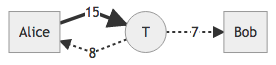
\includegraphics[scale=0.7]{ringtx}
\caption{A \textit{ring stealth transaction}}
\label{fig:ringtx}
\end{figure}

This commitment is represented by the formula: 

$R_{ct}=xG + aH(G)$

In the formula, $a$ is the amount sent out in the transaction, $x$ is a computed random value. By publishing the value of $R_{ct}$ to the network as an output, the network will be capable to verify the legitimacy of the submitted transaction. This technology goes on top of the already untraceable (Stealth) addresses used by the $x2x$ blockchain, and anonymous networking used to give full anonymity to the nodes involved.

In the $x2x$ Network, RingCT is used by default for all transactions except those used to participate to the sortition for Block Generator (which are normally \textit{ring signed}). This is merely a detail, though, considering that an external observer would not be able to tell these two kind of transactions apart from each other.

\subsubsection{Future Development: Bulletproof Transactions}

Initially, non-interactive proof of knowledge base on [Fiat-Shamir heuristic \cite{Shamir} have been taken into consideration in order to conceal transaction's information such as sender and amount. However, it quickly appeared that technologies developed on top of its concept such as zk-SNARKs \cite{zcash} require prohibitive computational power and time of processing for transaction generation. Even the more recent zk-STARKS \cite{starks}) revealed impractical to integrate in $x2x$ because of the problematic hurdle of needing extremely bulky verification proof (as big as several hundreds of kilobytes), although solving the problematic reliance to a trusted third-party for system setup and being substantially simpler than zk-SNARKS in terms of cryptographic primitives (they do not make use of Elliptic Curves, nor Public Key cryptography). 

The most promising advancement in the field of transaction confidentiality is probably given by the so-called Bulletproof Transactions \cite{bulletproofs}, which would appear to provide a substantial improvement over RingCT in terms of cryptographic proof size. At the time of this writing, first tests show a tenfold reduction in size and verification times (although still not reaching the same level of efficiency if compared to a zk-SNARK proof). Given the "pluggable" nature of $x2x$ core, the underlying software for transaction generation will be kept flexible through a plugin architecture in order to facilitate the adoption of a future implementation of Bulletproof Transactions as soon as an emerging library will prove stable enough for integration.

\subsection{Cryptographic Accumulator}
\label{sec:Cryptographic-Accumulator}
The set of algorithms known as cryptographic accumulators have been developed to allow hashing of a finite and potentially large set of values into a single succinct value, called the Accumulator. The algorithm enables efficient computation of a witness for every accumulated input that proves its membership in the accumulator. A dynamic accumulator is a special kind of accumulator which permits efficient input addition and deletion where the computation costs of these operation is independent on the number of values added or deleted. As such, it is a space and computational time efficient data structure initially developed for testing membership. 

Formally, a dynamic accumulator is a tuple of algorithms defined as follows:

\begin{itemize}
\item  $\textrm{Generate}(1^k)\rightarrow (sk_{acc}, pk_{acc})$: Given a security parameter $k$ return a (private, public) key pair. Notice that the parameter $k$ is sensitive information (trapdoor) which could deterministically recreate the private key  
\item  $\textrm{Eval}((sk_{acc}, pk_{acc}), \chi) \rightarrow (acc_\chi, aux)$: Probabilistic algorithm that gets the key pair and a set $\chi$ to be accumulated and returns the accumulator and some auxiliary data
\item  $\textrm{WitnessCreate}((sk_{acc}, pk_{acc}), acc_\chi, aux, x_i)\rightarrow wit_x \lor \bot$: Creates a witness $wit_x$ if $x_i \in \chi$, $\bot$ otherwise
\item  $\textrm{Verify}(pk_{acc}, acc_\chi, wit_x, x_i)\rightarrow wit_x\space \textrm{is a witness for }x_i$: This is the actual membership verification
\item  $\textrm{Add}(sk_{acc}, pk_{acc}, acc_\chi, aux, y_i)\rightarrow acc_{\chi'} \lor \bot$ : If the element $y_i$ is not already in the set $\chi$, returns the updated accumulator $acc_{\chi'}$ with $\chi' \leftarrow \chi \space \bigcup \space \{y_i\}$ 
\item  $\textrm{Delete}(sk_{acc}, pk_{acc}, acc_\chi, aux, y_i)\rightarrow acc_{\chi'} \lor \bot$ : If the element $y_i$ is in the set $\chi$, returns the updated accumulator $acc_{\chi'}$ with $\chi' \leftarrow \chi \space \backslash \space \{y_i\}$
\item  $\textrm{WitnessUpdate}((sk_{acc}, pk_{acc}), wit_x, aux, x_i)\rightarrow wit'_x \lor \bot$: Updates the witness for $x_i$ in case it has been added or deleted ($aux$ describes which of the two)
\end{itemize}

Different technologies exist that implement Accumulators with different level of computational efficiency and security requirements. Currently, $x2x$ is experimenting to achieve the best trade-off between a decentralized choice and efficiency of Accumulator technology. Following are the technologies under evaluation.

\subsubsection{RSA Accumulators}

Abundant literature has been developed regarding many different Accumulators, particularly the so-called RSA Accumulators. Considering \textit{strong RSA setting}, RSA accumulators (e.g. Carmenish's and Lysyanskaya's Dynamic RSA Accumulator \cite{accumulators}) are based on one-way RSA function for a suitably calculated $N =pq$ where $p$ and $q$ are sample primes with polynomial dependence on the security parameter $k$ and therefore are effectively the accumulator's \textit{trapdoors} which need to be \textbf{destroyed} immediately after parameters are generated. As an alternative, the employment of RSA-2048 could be used to circumvent the need for developers to know the security parameters and act as trusted party, considering that the related security parameter $k$ is claimed to be destroyed and no factoring solution to the RSA-2048 number has been found for the past 25 years \footnote{https://en.wikipedia.org/wiki/RSA\_Factoring\_Challenge}, despite a 200,000 incentive offered.

$acc_\chi \leftarrow g^{a} mod\space N$ // The set of members $a =\{a_1, .., a_n\}$ is compactly represented by the accumulator
$acc_\chi = g^{\prod{a \in \chi}}\\wit_i \leftarrow g^{(a_1, .., a_{i-1}, a_{i+1}, .., a_n)} mod\space N$

\subsubsection{Expressive Bilinear Accumulator}

Under such security assumption, dynamic Accumulator schemes from \textit{bilinear pairings} have been developed in the literature. Among those, an expressive \textit{zero-knowledge} set Accumulator has been formalized by Zhang, Katz and Papamanthou \cite{zeroaccum} capable of providing succinct proofs for a large collection of operations over accumulated sets, among which it is of particular interest the $\textrm{SUM}$ operation, which could find application for rapid and zero-knowledge calculation of accumulated \hyperref[sec:Cryptographically-Committed-Provisioners]{Provisioners stakes}.

However, similarly to RSA, also bilinear pairing accumulators present the drawback of relying on the security parameter $k$.

\subsubsection{Elliptic Curve Multiset Hash}

Shepard, Tibouchi and Aranha \cite{ecmh} teach of a new and efficient method to "\textit{associate a hash value to arbitrary collections of objects (with possible repetitions) in such a way that the hash of the union of two collections is easy to compute from the hashes of the two collections themselves:  it is simply their sum under a suitable group operation}". This association is the basis for an Elliptic Curve Multiset Hash which constructs a homomorphic multiset hashing on top of efficient \textit{BLAKE2} hash function and binary elliptic curve encoding. This allows for incremental/parallel computation of a hashing function for various applications including efficiently testing for subgroup membership. This makes ECMH an appealing alternative to the other known algorithms to construct Accumulators, especially since the method is unencumbered with the necessity of a trusted setup.

\section{Segregated Byzantine Agreement}
\label{sec:SBA}

The $x2x$ blockchain is built upon a novel consensus mechanism, called \textit{Segregated Byzantine Agreement} (SBA$\large\star$), engineered to provide the best possible tradeoff between security, efficiency and flexibility. 

SBA$\large\star$ complements the idea of \textit{Cryptographic Sortition,} \textit{Player Replaceability} and \textit{Ambiguity Resilience} (firstly introduced by the BA$\large\star$ consensus developed by Micali and the MIT CSAIL \cite{algorand}) with the new concepts of \textit{stealth time-locked transactions} as a method for Sybil resistance and \textit{non-interactive verifiable shared secret} scheme to implement a simple but secure $\textrm{(t,n)-threshold secret}$ sharing for keeping sortition auditable solely by a rotating set of \textit{pre-block Verifiers}.

In order to both improve network and block-generation efficiency and privacy of transacting peers, SBA$\large\star$ allows only normal transactional nodes to compete for block-generation, while it restricts the computationally and network intensive tasks associated with verification, voting and notarisation (VVN operations) to non-transactional nodes called \textit{Provisioners}. Provisioners harden the $x2x$ Blockchain by decreasing network communications across VVN operations, improving the time-to-finality through a notarisation process, decreasing the probability of network partitioning and contributing to the overall availability of $x2x$ Network.

Furthermore, they contribute distributed storage infrastructure in the $x2x$ On- Offline File Transfer, and enable runtime payments of high QoS transmission by handling \textit{state channels} for communicating peers through a novel mechanism of Secure Tunnel Switching.

\paragraph{BA$\large\star$}

Cryptocurrencies powered by message-passing Byzantine Agreement (BA$\large\star$), use cryptographic sortition in order to carry out the functionalities of block proposals, validations and subsequent insertion into a tamperproof sequence of blocks.

In its essence, each node of the network, while collecting (and further relaying) pending transactions, runs a computationally lightweight process that yields in a pseudo-random fashion which role such node should assume in the operations of production and validation of a new block. The great advantage of BA$\large\star$ compared to other consensus mechanisms based upon \textit{proof-of-work} or \textit{proof-of-stake}, lays primarily in avoiding any possibility of forking the Blockchain and thus preventing any ambiguity about which branch will become the dominating one.

This translates into the appealing property of achieving transaction "finality" as soon as consensus is reached for a block. In the best case scenario this happens after 2 rounds of non-interactive sortition. In the worst case scenario (weak network synchrony controlled by adversaries for a long but  bounded period of time), BA$\large\star$ achieves block finality after 9 rounds.

BA$\large\star$ consensus is a very convincing engine for powering open cryptocurrencies which do not require privacy. The election of Block Generator and Block Voter requires the total weights available in the system and each \textit{sortition candidate}'s balance to be public and known by all peers in order to allow blocks proposed by higher priority members to be propagated within the network and validated by multiple voting committees.

This is problematic for a privacy-oriented digital currency such as $x2x$ which strive to protect the data of the transacting actors. SBA$\large\star$ therefore focuses primarily on the privacy of transactional nodes while keeping auditable (but not public) only essential information about nodes participating in block generation, validation and notarisation.

\subsection{Consensus Outline}

The BA$\large\star$ algorithm has been developed in a direction unsuitable for $x2x$ because transactions are supposed to be propagated in clear, nodes do not keep private state except their private keys and there is no measure to prevent every node in the network to learn of every other node's balance, IP address and, ultimately, providing a mere pseudonimity to protect their identity.

We propose here a new approach that evolves BA$\large\star$ into what we call SBA$\large\star$ (as in \textit{Segregated Byzantine Agreement}$\large\star$) which finally renders the consensus mechanism an outstanding choice for privacy-oriented currencies (such as $x2x$) due to its quick finality mechanism, minimal amount of computation required and speed in block production.

SBA$\large\star$ foresees different subsequent cyclic phases, all of which are non-interactive, with the sole exception of the \textit{Validation}, where the $\textrm{NIVSS\_Reconstruct}$ requires $O(1)$ communications to complete.
\paragraph*{Block Generation Sortition} Run by nodes with a time-locked stake called \textit{Block Generator} candidate (or simply a "\textit{candidate}"). During this phase the candidates run the VRF, calculate their priority, run the Non-Interactive Verifiable Shared Secret Protocol and propagate a \textit{pre-block} (which is a block proposal that still needs to get through various round of consensus and gets decorated with additional meta-data along the way) together with the various proofs.

\paragraph*{Default Block Generation Sortition} 
Run by Provisioners in parallel to the Block Generation Sortition. In the eventuality that the Block Generation Sortition produces no \textit{candidate} with priority higher than zero or the Validation phase fails, Provisioners run the classic BA$\large\star$ Sortition algorithm to supply a \textit{default pre-block}.  
\paragraph*{Validation}
Run by a subset of \textit{Provisioners} called \textit{Verifiers}. \textit{Verifiers} run the \textit{Secret Reconstruction Protocol}, validate the priority information of the highest priority candidate and either sign on the pre-block proposal of the \textit{candidate} or a \textit{default pre-block}. Additionally, the \textit{Verifiers} validate the witness $wit_P$ of candidate Provisioners committing their stake to the \hyperref[sec:Cryptographically-Committed-Provisioners]{Accumulator} if any. In this case, this information gets added to the pre-block
\paragraph*{Voting}
A number of rounds each of which run by a different subset of \textit{Provisioners} called \textit{Voters}. BA$\large\star$ proves that the amount of round is optimistically 4 for a strongly synchronous network and 9 for a weakly synchronous one with a strong adversarial presence controlling the network (albeit for a finite period of time)
\paragraph*{Notarization}
The \textit{Voters} which reached voting consensus on the pre-block are called \textit{Notaries}. Their public key is added to the pre-block and they play the role of \textit{Verifiers} in the next block's Validation phase. The pre-block is then turned into an official block by the Notaries who add \hyperref[sec:Block-Reward]{the Block Reward information}.

\subsection{Verifiable Random Function}
\label{Verifiable-Random-Function}
The cryptographic sortition is implemented through the so-called Verifiable Random Function (VRF). Formally, for a generation algorithm $G\small{EN}$ producing the key pair $(P_k, S_k)$, a proving algorithm $P\small{ROVE}_{Sk}\normalsize(x)$ which outputs a pair of function value and proof of correctness ($F_{Sk}(x), \pi_{Sk}(x)$), a \textbf{VRF} is a function for which it exists a verification algorithm $V\small{ER}_{Pk}\normalsize(x, y, \pi)$ which verifies that $y=F_{Sk}(x)$ using proof $\pi$.

In practice a node running a VRF can prove the output it received by propagating $\pi$ together with the VRF result. This way a node, by running a VRF and communicating its output, can convince its peers in a non-interactive fashion (meaning without talking to anyone else in the network) whether he has been selected by "the cryptographic sortition" to play a specific role in the current block creation round.

The roles are either \textit{Block Generator\textit} or \textit{Block Verifier}. The elected node will then proceed to perform the steps foreseen by its role independently from all the other nodes (regardless of their role) and thus propagate the result of such operations to the network together with their allotment proof as outputted by the VRF. The nodes forfeit their role and become irrelevant to the consensus as soon as they communicate with the network. This way, the algorithm makes it virtually impossible for an adversary to target nodes participating in the block election or transaction validation. Only a small fraction of the nodes each round get randomly selected.

The likelihood of positive VRF output depends on a weight correlated to the amount of digital currency committed by a node. In \textit{BA$\large\star$} this is the public balance of each node, in SBA$\large\star$ this depends on the sortition role (i.e. Block Generators commit a payment while Provisioners commit a stake). Regardless of the type of commitment, the weight mechanism is used to prevent Sybil attacks since it renders probabilistically and economically disadvantageous for a node to replicate itself over several different sybil processes, since such behaviour would actually decrease its chance of winning the ballot.

\begin{figure*}
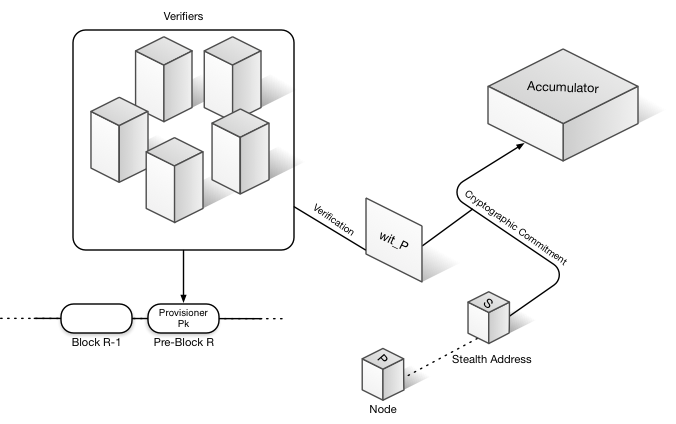
\includegraphics[scale=0.5]{Provisioners}
\caption{Provisioners setup}
\end{figure*}

\subsubsection{VRF And Sortition Procedure}

Through VRF sortition, a number of Block Generator candidates are selected each round. The candidates propagate their proposed block together with the VRF output, which includes the proof of winning the sortition together with the priority given by the digital currency balance of the node. Peers collect and propagate gossiped packets, forwarding solely the message with the highest priority and discarding all the others. The amount of time peers are supposed to collect messages is usually part of the protocol configuration and is suggested to be 5 seconds.

At the end of this period, peers which did not receive a message propagate an empty block (which is a perfectly valid outcome of the consensus). From a security perspective, an adversary could orchestrate an attack by deceiving peers into propose different blocks. However, this attack would fail unless the adversary would have the highest priority in a round and if the number of honest Provisioners are also lesser then 2/3rd.

\subsection{Cryptographically Committed Provisioners}
\label{sec:Cryptographically-Committed-Provisioners}
One approach to protect the stake information was the employment of Order Preserving Encryption and Homomorphic Cypher \cite{alec}, which would have theoretically allowed for priority comparison without revealing the balance of the different nodes. This approach however has been discarded because it is susceptible to binary search attack. In fact, by exposing priority information, any attacker with access to the oracle could ultimately obtain information about the original balance of a node simply by performing multiple comparisons with the hash of a known number. Additionally, every node in the network is required to perform validation on the packets it receives.

Since the priority of the Block Generator is an input parameter for validating its VRF’s output, the measures required to provide access to such datum in a secure setting would result in an unacceptable degradation of performances and increase in complexity.

Instead, in the attempt to obtain the best trade-off between efficiency and anonymity, the system restricts the opportunity to perform VVN operations solely to non-transactional nodes called \textit{Provisioners} organized in elected subsets which form different committees throughout the algorithm rounds. In order to being eligible to be a Provisioner, a node $P$ uses a non-interactive \hyperref[sec:Cryptographic-Accumulator]{cryptographic commitment} to bind a predefined minimum amount of $x2x$ coins $C$ into a collective anonymous escrow and creating a $spend$ transaction toward a \textit{stealth address} obfuscating $P$'s address. Such $spend$ transaction is kept concealed until the node is ready to cash back its stack and quit its role as Provisioner.

The system verifies through an efficient (i.e. within \textit{polynomial-time}) \textit{non-interactive zero knowledge proof}  $wit_M$ that $P$ actually committed its stack in the Accumulator. This means that as soon as the Provisioner commits its stake to the Accumulator, it announces itself as a Provisioner to the network by gossiping its public key, its $x2x$ Network Address and $wit_P$. The drawback of relying on a trusted setup is circumvented by using the RSA-2048.

Also, the notoriously big size of spend proof (estimated to be 45kb in the Zerocoin whitepaper \cite{zerocoin}) is not problematic in the case of Provisioners since their stake is meant to be in a long-term escrow. This is easily enforceable at protocol level.



\subsection{Non-Interactive Verifiable Shared Secret Protocol}

Verifiable Secret Sharing (VSS) is a cryptographic protocol designed to allow a dealer to decompose a secret in $n$ fragments and share them publicly to $n$ peers (players) so that only a subset (\textit{threshold}) $t$ or those fragments are needed to reconstruct the original secret. In a VSS, through the addition of auxiliary information, players can verify reception of a "valid" fragment without acquiring any knowledge of the initial secret.

The Non-Interactive Verifiable Secret Sharing Protocol is $x2x$ variation of the Simplified VSS protocol of Gennaro, Rabin and Rabin \cite{grr}. In our protocol, the \textit{dealer} does not communicate directly with the \textit{players} but can only rely on multiple untrusted message relayers as it is the case using the $x2x$ gossip protocol. The protocol foresees a \textit{sharing phase} () and a \textit{Reconstruction Phase}. The constant term $s$ of $f(x)$ is the secret. The second polynomial $r(x)$ is used to generate $t$ independent random strings used to commit to the shares.

The verification performed by player $P_i$ after decrypting its share $S_i$ from the share vector $S$, with its own private key $sk_i$ is trivially to recompute $\mathcal{A}_i = \mathcal{C}(\alpha_i, \rho_i)$ and check that the equation holds. $\mathcal{C}(x, r)$ is a commitment hash function such as $\textrm{Skein}$ or $\textrm{SHA-3}$.

    \begin{algorithm}
        \caption{Share secret in a verifiable and non-interactive way}
        \begin{algorithmic}[1]
            \Procedure{NIVSS\_Share}{$s, V$} \Comment{$s$ is a secret, $V$ a list of $n$ Verifiers $pk$}
                \State $f(x) = s \space + a_1x^1 + .. + a_tx^t$ \Comment{$f(x)$ is a random polynomial}
                \State $r(x) = r_0 + r_1x^1 + .. + r_tx^t$ \Comment{$r(x)$ is a random polynomial}
                \State $S = \{\}$
                \State $\mathcal{A} = \{\}$
                \For{each player $i$ in $V$}
                	\State $(\alpha_i, \rho_i) \leftarrow (f(i), r(i))$
                	\State $S_i \bigcup = \{Enc_{pk_i}(\alpha_i, \rho_i)\}$
                	\State $\mathcal{A}_i \bigcup = \{\mathcal{C}(\alpha_i, \rho_i)\}$
                \EndFor
                \Return{$\langle S, \mathcal{A} \rangle$}
            \EndProcedure
        \end{algorithmic}
    \end{algorithm}

    \begin{algorithm}
        \caption{Reconstruct the secret (View-Key)}
        \begin{algorithmic}[1]
            \Procedure{NIVSS\_Reconstruct}{$S, \mathcal{A}$}
                \State $\langle\alpha_p, \rho_p\rangle \leftarrow Dec_{pk_p}(S[p])$
                \State Sig${^p}_{\alpha_p||\rho_p} \leftarrow \textrm{Sig}_{sk_p}(\alpha_p||\rho_p)$
                \State $\textrm{Gossip}_V(\langle\alpha_p, \rho_p, \textrm{Sig}{^p}_{\alpha_p||\rho_p}\rangle)$ \Comment{propagate share solely to other verifiers}
                \State $\mathcal{F} \leftarrow \{\}$ \Comment{List of all shares (i.e. points of $f(x), r(x)$)}
                \BState \textbf{loop} \emph{onShareReception}:
                \State $\langle\alpha_i, \rho_i, \textrm{Sig}{^i}_{\alpha_i||\rho_i}, \mathcal{H^i(b_c)}, \textrm{Sig}_{pk_c}(b_c)\rangle \leftarrow \textrm{INPUT}$
                \If{$\mathcal{H}^p(b_c) \neq \mathcal{H}^I(b_c)$} \Comment{If different pre-blocks...}
                	\State \textbf{return} \textit{Complaint}$_{pk_c}$ \Comment{...candidate is dishonest}
                \ElsIf{$\textrm{Vf}(\textrm{Sig}{^i}_{\alpha_i||rho_i})$}                	
                    \State $\mathcal{F} \bigcup = \{(\alpha_i, \rho_i)\}$
                    \If{$\textit{length}(\mathcal{F}) \geq t + 1$}
                    	\State interpolate $\hat{f}(x)$ and $\hat{r}(x)$ that touch all $\mathcal{F}$ 
                        \State \textbf{return }$\hat{f}(0)$
                    \EndIf
                \Else
                	\State \textbf{return} \textit{Complaint}$_{V_i}$
                \EndIf
                \BState \textbf{end loop}
                \State \textbf{return await} \emph{onShareReception}                
            \EndProcedure
        \end{algorithmic}
    \end{algorithm}


\subsection{Block Generation Sortition}

A node that wishes to participate in the Sortition (and become a \textit{Block Generation candidate} or simply "\textit{candidate}") is first required to lock an arbitrary amount of $x2x$. A \textit{time-locked transaction} is a special transaction where the output is un-spendable for a predetermined period of time. In order to participate to the Sortition lottery for proposing a block, the candidate performs a time-locked transaction toward a Stealth Address $s\_addr_{pk^2}$ where recipient party's key is the public key $p_k$ (which is thus used twice). Such a transaction is indistinguishable from the normal others. When propagating the result of the sortition, the \textit{Block Generator candidate} runs the dealer part of the NIVSS Protocol to encrypt the meta-data composed by the \textit{view-key} for the time-locked transaction and by the locking period expressed in number of blocks into a shared secret. Thus, it propagates such secret, together with the proof for the NIVSS and the hash of the meta-data signed with the node's private key $s_k$. 

Following is a description of the Block Generator Sortition. Whereas: 

\begin{itemize}
\item VRF is the Elliptic Curve Verifiable Random Function \ref{Verifiable-Random-Function} as described in NSEC5 For Elliptic Curves \cite{ecurves}
\item $(pk, sk)$ are the public/private keys of the node with a candidate Block Generator
\item $seed$ is a public random seed chosen and propagated together with the last block
\item $\Theta$ is the maximum number of candidate Block Generators per sortition
\item $\pi$ is the proof allowing anyone knowing $pk_i$ to check that the hash corresponds to the input parameters of the VRF
\item $vk_{tx}$ is the Block Generator's view-key of a stealth time-locked transaction
\item $w_P$ is the sum of all balances of all Provisioners
\item $W$ is the amount of circulating $x2x$
\item $V$ is the list of $n$ validators identified by their public key $pk_i$
\end{itemize}

In Algorithm \ref{alg:sortition} we find the pseudocode for the Block Generator sortition procedure for a node $N$.

    \begin{algorithm}
        \caption{Sortition for generating the pre-block with priority $j$}
        \label{alg:sortition}
        \begin{algorithmic}[1]
            \Procedure{BlockProposerSortition}{$seed, \Theta, w_P, W, V$}
                \State $\langle hash, \pi\rangle \leftarrow VRF_{node.sk}(seed)$
                \State $p \leftarrow \frac{\Theta}{W-w_P}$ \Comment{$p$ is the maximum probability to be selected in $N$ extractions}
                \State $j \leftarrow 0$
                \State $(n, t) \leftarrow time\_locked(s\_addr_{node.pk^2})$ \Comment{tuple of $n$ $x2x$ and $t$ nr of blocks}
                \While{$\frac{hash}{2^{len(hash)}} \notin [ \sum_{k=0}^j Pr(k;n,p), \sum_{k=0}^{j+1} Pr(k;n,p))$}
                	\State $j \textrm{++}$
                	\State $\langle S, \mathcal{A} \rangle \leftarrow \textrm{NIVSS\_Share}(vk_{tx}||t, V)$
                	\State $\sigma_{n,t}=\textrm{Sig}_{node.sk}(vk_{tx}|| t)$
                \EndWhile
                \Return{$\langle hash, \pi, j, \sigma_{n, t}, S, A \rangle$}
            \EndProcedure
        \end{algorithmic}
    \end{algorithm}


A node runs the sortition process to become a Block Generator by
calculating the pseudo-random \(hash\) and the proof \(\pi\) by feeding
the VRF its secret key \(s_k\) and the \(seed\) calculated and
propagated when last block was chosen. The VRF returns a \(hash\) which
is essentially a value with uniformly distributed probability between 0
and \(2^{len(hash)} - 1\) where the \(len\) function is the bit-length
of the \(hash\). The priority \(j\) for the node is calculated by
considering each unit of \(x2x\) in the \emph{time-locked transaction}
performed toward the stealth address \(s\_addr_{pk^2}\) as an
independent runner for the Block Generation lottery. This means that for
each node \(N\) participating in the sortition with a \emph{time-locked
payment} of \(n\) amount of \(x2x\) there are exactly \(n\) runners at
every selection round.

The probability for obtaining \(k\) selections out of \(n\) extractions
follows the binomial distribution
\(Pr(k; n, p) = \left( \begin{array}{c} n \\ k \end{array} \right)p^k(1-p)^{n-k}\)
where the sum of all probabilities \(\sum_{k=0}^n Pr(k; n, p)\) is
naturally 1. The set representing all possible probability values
\([0, 1)\) gets split into adjacent intervals
\(I^j = [\space \sum_{k=0}^j Pr(k;n,p), \sum_{k=0}^{j+1} Pr(k;n,p)\space  )\)
for \(j \in {0, 1, ..., n}\). If \(hash/2^{len(hash)}\) falls in the
intervals \(I^j\), then \(j\) is the priority of the node's sortition
and it is verifiable by knowing the VRF's output \(hash\) (proven by
\(\pi\)) and the amount \(n\). While in \emph{BA}\(\large\star\) \(n\)
is the information about a node's entire balance, in
\emph{SBA}\(\large\star\) this amount is instead encrypted by the node
and shared among the \emph{Verifiers} using the NIVSS algorithm and kept
verifiable solely by a threshold t of the n members of the Verifier
Committee.

Differently from \emph{BA}\(\large\star\), in \emph{SBA}\(\large\star\)
the probability of obtaining a total amount of \(\Theta\) positive
extractions is 1 only if all nodes participate to the sortition with
their whole balance. This is seldom the case and therefore the
probability that no candidate get selected to propose a block is greater
than zero. To obviate to this eventuality and still produce a block in
case a dishonest Block Generator gets caught, Provisioners run their own
parallel Block Generator sortition as a fallback scenario for those
cases. Also, to mitigate the potentially reduced probability to generate
a successful sortition with multiple candidates, \(\Theta\) is chosen to
be substantially higher than the \(\tau\) parameter of
\emph{BA}\(\large\star\).

\subsection{Verification --- Pre-Block Propagation}

During the gossip procedure, each node relays solely the pre-block with
the claimed highest priority (Provisioners will also gossip the default
pre-block to the other Provisioners), while dropping all other pre-block
proposals. In \emph{SBA}\(\large\star\), protection from sybil attacks
is granted by the \emph{time-locked payment} made by the \emph{Block
Generator candidate} which is not in clear. Therefore nodes and
Provisioners other than \emph{Verifiers} could only perform validation
on the VRF result \(hash\) and the proposed pre-block. They do not
engage in priority validation, which is entirely demanded to the
\emph{Verifiers}. This has the positive side-effect to perceivably
decrease network latency during gossip operations.

\emph{Verifiers} run the \(\textrm{VerifyBlockProposerSortition}\) in
order to reconstruct the \emph{view-key} and the \emph{time-locked
transaction} propagated by the Block Generator candidate and be able to
validate the claimed priority. Depending on the outcome, their either
sign and propagate the candidate's pre-block or the default pre-block.
This does not really require consensus since the propagated pre-block is
a mere result of the validation operation, which gets further audited by
the different \emph{Voter Committees}. As such the probability for
propagating mismatching pre-blocks is negligible. In the future we will
explore the possibility to use
\href{https://www.iacr.org/archive/asiacrypt2010/6477343/6477343.pdf}{Probabilistic
Checkable Non-Interactive Zero Knowledge Proofs} to propagate a very
efficient proof of validation without revealing the candidate's
\emph{view-key} any further than the \emph{Verifiers}.

Whereas:

\begin{itemize}
\item
  \(j_c\) is the claimed candidate's priority
\item
  \(t_{block}\) is the time when the pre-block has been produced
\item
  \(pk_c\) is the \emph{candidate's} public key
\item
  \(ctx\) represents an object encapsulating the state of the ledger
\item
  \(b_{c}\) is the \emph{tuple} of the pre-block candidate hash
  \(\mathcal{H}(block)\) and the transaction list \(tx_{block}\)
\item
  \(b_{default}\) is the default pre-block propagated by the appropriate
  Provisioner's committee
\end{itemize}

    \begin{algorithm}
        \caption{Verify and propagate pre-blocks}
        \begin{algorithmic}[1]
            \Procedure{PropagateVerifiedBlock}{hash, $\pi, ctx, pk_{c}, j_{c}, b_{c}, S, \mathcal{A}$}
                \State $\langle vk_{tx}, t\rangle \leftarrow$ NIVSS\_Reconstruct$(S, \mathcal{A})$
                \State $n \leftarrow $ \textit{extractAmount}($vk_{tx}$)
                \If{$\neg \textit{VerifyVRF}_{pk}(hash, \pi, ctx.seed)$}
                    \State \textit{Gossip $Complaint_{pk_c}$, validation data and signed $b_{default}$}
                    \Break
                \EndIf
                \State $p \leftarrow \frac{ctx.\Theta}{ctx.W-ctx.w_p}$
                \State $j \leftarrow 0$
                \While{$\frac{hash}{2^{len(hash)}} \notin [ \sum_{k=0}^j Pr(k;n,p), \sum_{k=0}^{j+1} Pr(k;n,p) )$}
                    \State $j$++
                \EndWhile
                \If{$j \neq j_c \lor \neg (VerifyTx(b_c.tx_{block}))$ \\ $\lor\space(ctx.t_{last\_block} > b_c.t_{block})$ \\ $\lor\space\neg(VerifyBlock(ctx.seed_{pk}, b_c.\mathcal{H}(block)))$ }
                \State \textit{Gossip $Complaint_{pk_c}$, validation data and signed $b_{default}$}
                \Break
                \EndIf
            \State Gossip$(\langle node.pk, Sig_{node.pk}(pk_c, hash, \pi, j_{c}, b_{c}, vk_{tx}, t) \rangle)$
            \EndProcedure
        \end{algorithmic}
    \end{algorithm}

Verifiers already operate an implicit \textrm{Reduction} procedure
through the asynchronous function \textrm{onReception} within the
\textrm{NIVSS\_Reconstruct} procedure, which checks the shares as
well as the block and the hash propagated by the \emph{candidate}. As
taught by Turpin and Coan \cite{ebiza} two-step technique, such an implicit reduction of the problem
to reaching consensus on a binary choice (either the candidate's
pre-block hash or the default pre-block) is important to ensure
liveness.

\begin{figure*}
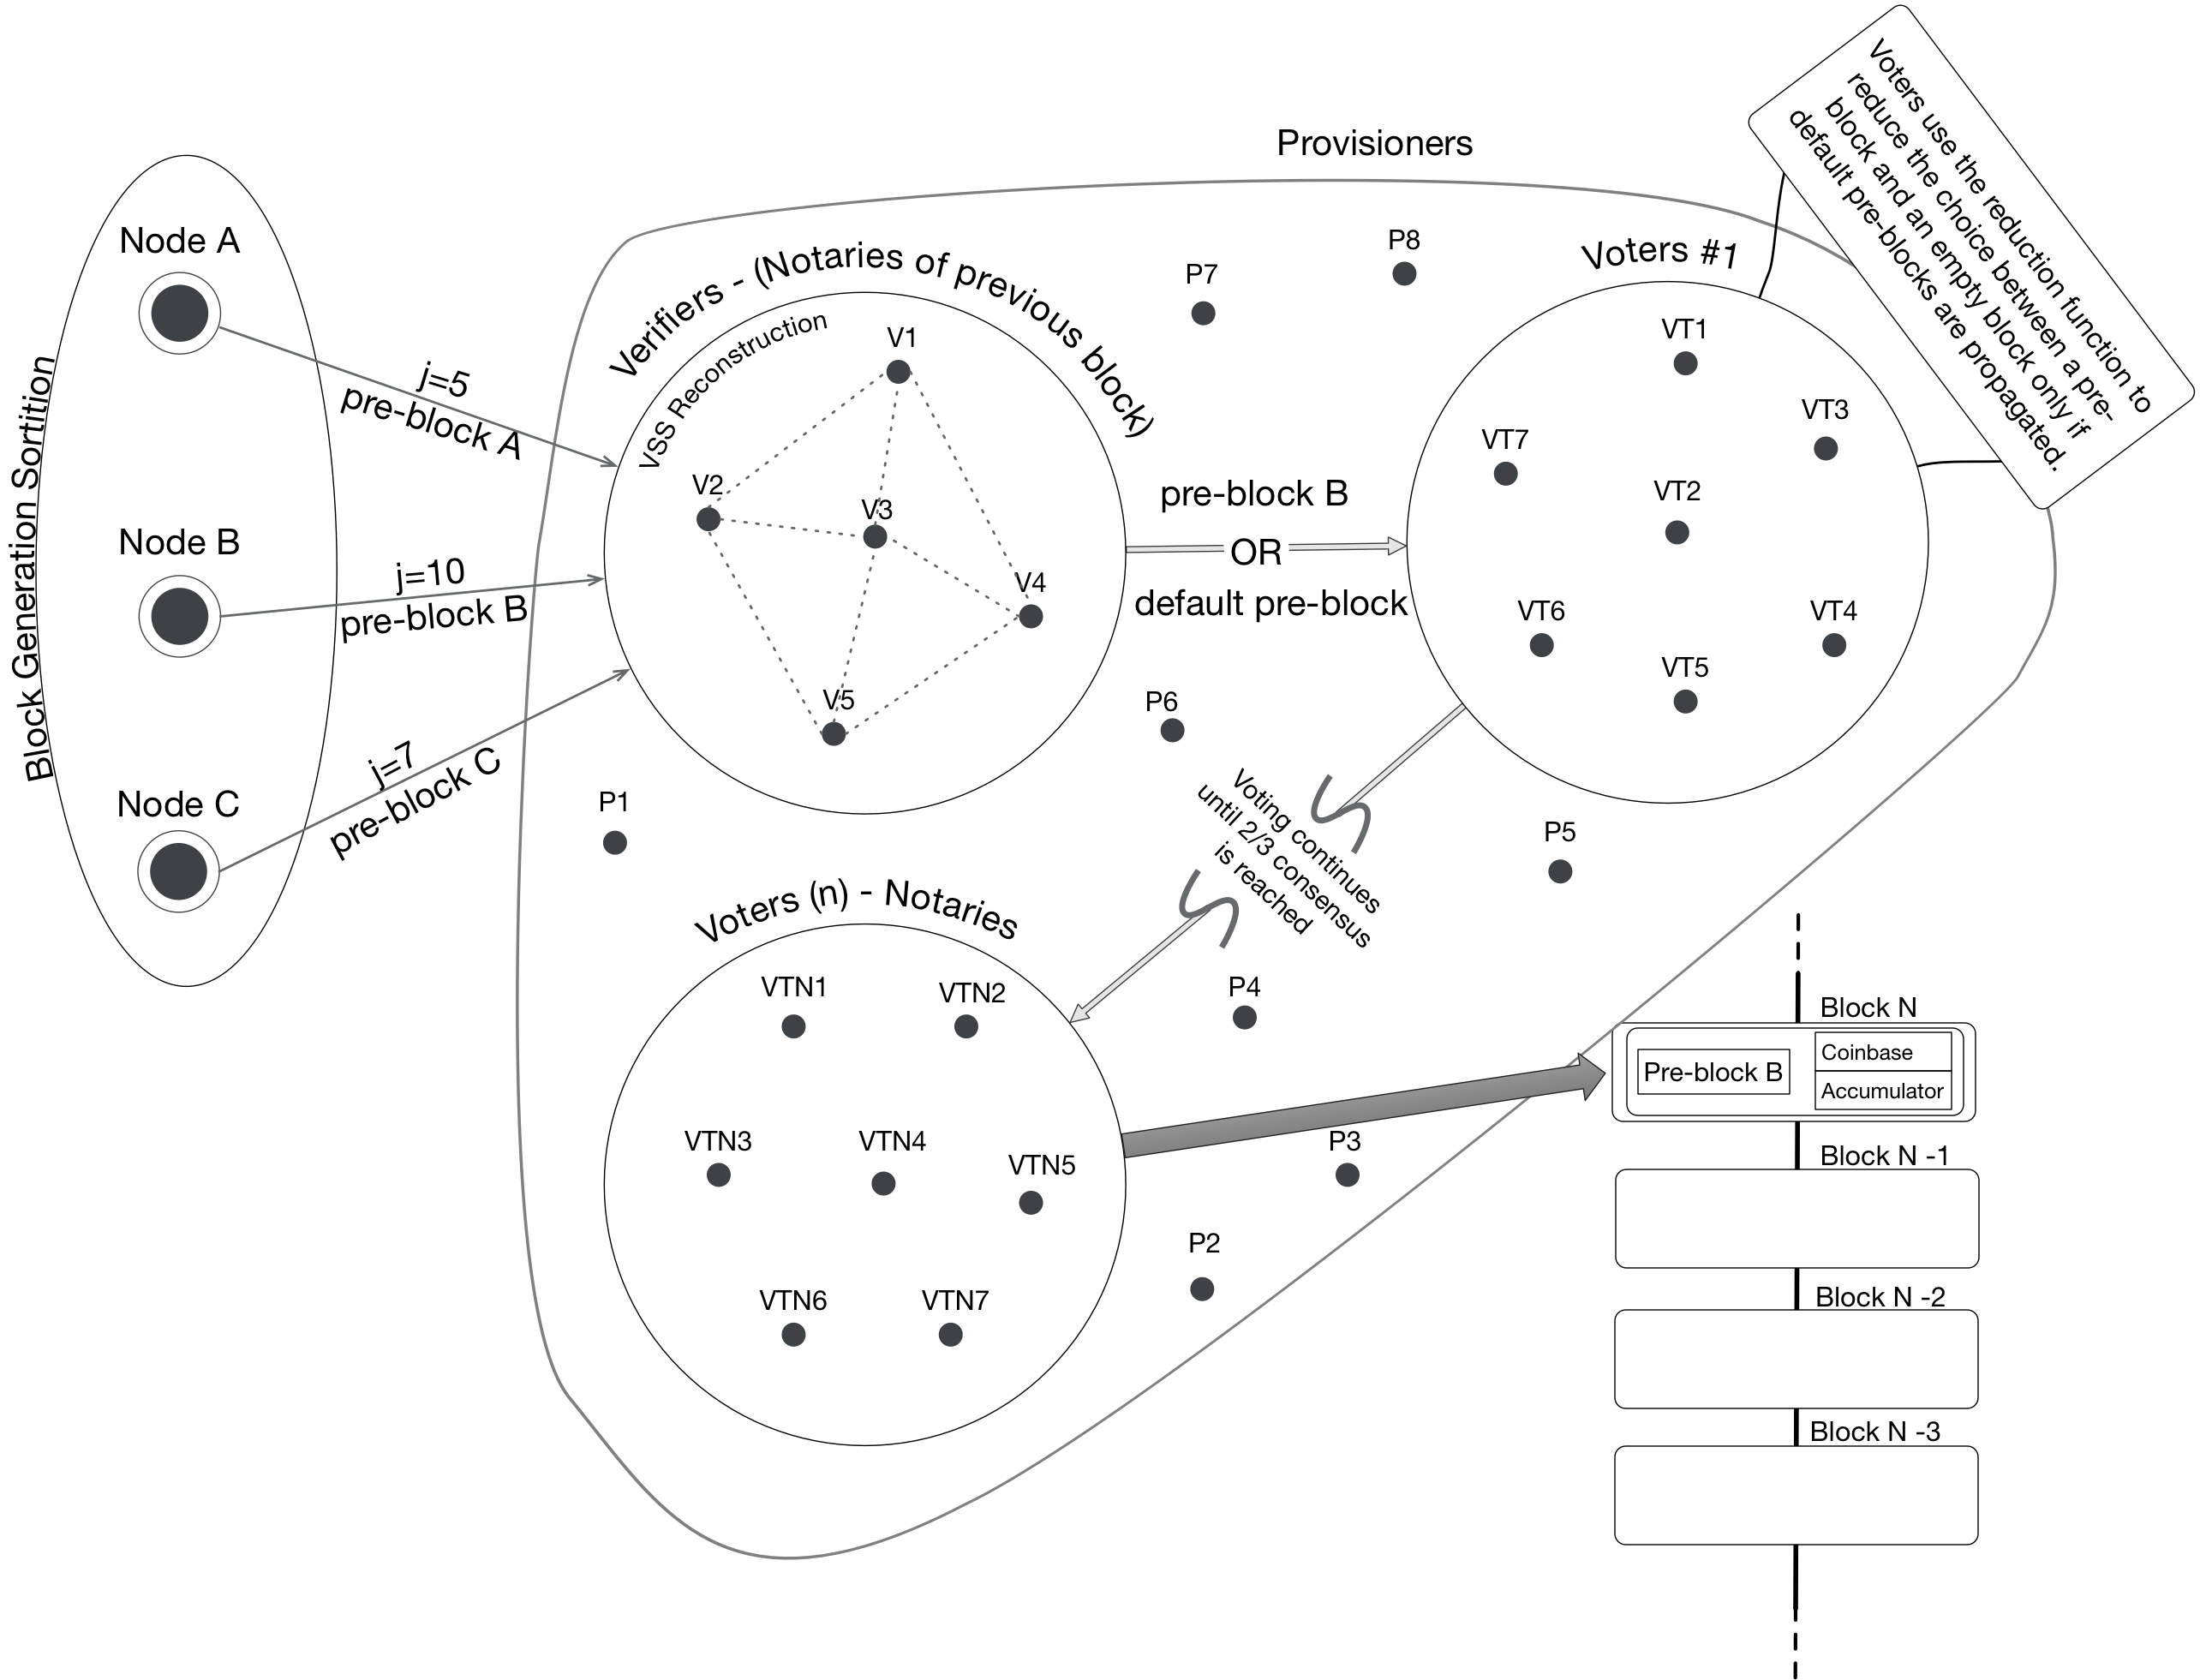
\includegraphics[scale=0.2]{sba}
\caption{SBA$\large\star$ at a glance}
\end{figure*}

\subsection{Voting On Blocks --- Voter's Sortition}

While nodes compete for generating the block, Provisioners other than
the \emph{Verifiers} run the Sortition procedure so to be appointed the
task of \emph{Voters} and reach Byzantine consensus over different
rounds of voting.

Block election happens through a set of steps, each
one requiring a different committee being formed by peers sorted through
VRF output with the voter's role. During each step, sorted nodes (and
only them) gossip their signed hash of the block together with block
round, step in the process and proof of sortition as outputted by the
VRF. Since voting is a task reserved to Provisioners, gossip during this
phase stays confined within the Provisioners' boundaries and is relayed
solely by Voters. As a result, the voting operations completes much
faster than all the others since there is no need to wait enough time
for messages to reach all extremities of the network.

Provisioners organised in subsequent elected \emph{Voting Committees} try to reach consensus (i.e. counting enough votes for either the pre-block hash or the empty block) by progressively raising the amount of votes for a pre-block or an empty block.

At each subsequent step, the votes casted during the step before remain
accounted for, while the new elected Provisioners cast new votes until
the required majority is reached. Intuitively, the convergence is
guaranteed by the fact that Voters which have already declared consensus
for a pre-block will not vote for any other value in the same round and
will keep proposing the same result until consensus converges.

\subsection{Notaries --- Block Rewards}
\label{sec:Block-Reward}

As soon as the \emph{Validators} reach consensus over a non-empty
\emph{pre-block}, they turn into \emph{Notaries} by running a
supplementary procedure aimed at generating a new block by hashing the
pre-block with a set of \textbf{coin-base} transactions. A
\emph{coin-base transaction} is basically a transaction with no input
which mints new \(x2x\) coins and spend them to the address of the
\emph{Block Generator}.

As opposed to Block Generators, Provisioners do not gain their reward by
winning the sortition procedure. Rather, at the end of each block an
amount of \(x2x\) coins is \emph{coin-based}, dependent on the stake
amount committed by the Provisioner to the Accumulator, independently
from whether they participated to the Block Committee or not. This
amount is thus spent toward the Provisioner's address.

Counterintuitively, the rewards paid are inversely proportional to the
staked amount (i.e. bigger stakes get proportionally less rewarded, in
respect to smaller stakes). This measure is novel and to the writers'
knowledge not a viable option outside of \(x2x\) Blockchain, where the
probability to win the sortition lottery and therefore take an active
part to the \emph{SBA}\(\large\star\) algorithm is not associated with a
reward, except the sole payment of the transaction fees.

The motivation
is twofold. Together with preventing the \emph{rich gets richer} scheme,
the intention is to create a counterposition between \textbf{power}
(intended as the capability to influence block generation by being
selected as part of the Block Committee) and \textbf{money} (intended as
the financial benefit acquired from running Provisioners). Considering
that \emph{SBA}\(\large\star\) is already protected from Sybil attack by
making it probabilistically disadvantageous to dilute a stack into
several balances, similarly, by reversing the proportion between rewards
and stake, the system prevents financially motivated participants to
benefit from organizing themselves into few Provisioner pools at the
expense of decentralization.

\begin{figure}
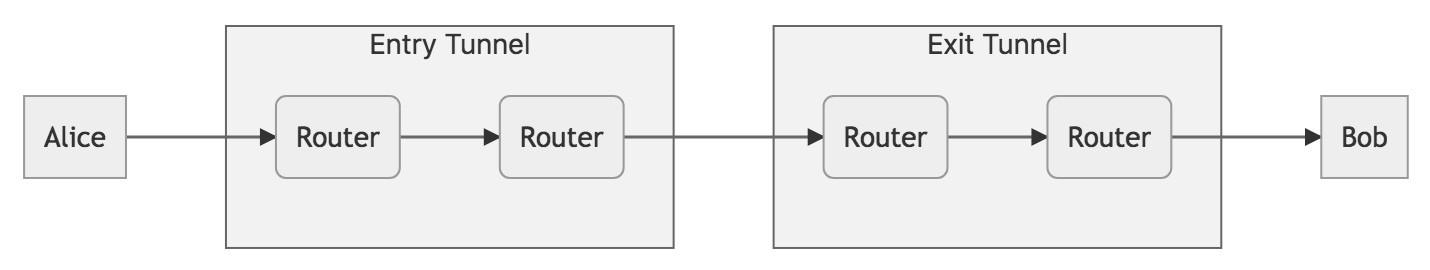
\includegraphics[scale=0.18]{tunnels}
\caption{$x2x$ tunneling}
\label{tunn}
\end{figure}


\section{\texorpdfstring{\(x2x\) Anonymous Network
Layer}{x2x Anonymous Network Layer}}


On the vast majority of blockchain implementations, network
communication protocols limits themselves to just embrace the privacy
standards we have in place today for our daily internet needs: TCP/IP,
UDP, SSL for encrypting communication channels to name a few.

While this can be considered acceptable for centralized environments or
platforms where user privacy is not the main proposition, the anonymity
and privacy requirements established with the \(x2x\) network impose the
adoption of technology offering at a much higher level of privacy
protection.

To achieve this goal, \(x2x\) is enabling full anonymity over its
decentralized network by integrating an advanced, custom bi-directional
routing, fully compatible with \href{https://geti2p.net/en/}{I2P}'s
\href{https://en.wikipedia.org/wiki/Garlic_routing}{Garlic-Routing}
technology for all its networking communications, but extending the
underlined protocol not only for the deployment of additional
functionalities (such as fully anonymous file transfer) but also for
allowing the default anonymous gossip protocol which powers the entire
\(x2x\) network.

The proposed architecture has been designed to render computationally
infeasible for an eavesdropper to tell apart \(x2x\) related traffic
from other network activities. Additionally, it should be very hard for
any network node to associate a \(Tx_{id}\) with the IP address of the
original initiator.

Compared to similar solutions, the \(x2x\) approach offers the following
benefits:

\begin{enumerate}
\def\labelenumi{\arabic{enumi}.}
\item
  Makes use of \emph{packet routing}, instead of \emph{circuit routing}.
  This means transparent load balancing of all networking message across
  peers, instead of a single tunnel.
\item
  Multiple packets are joined together in inconspicuous messages, making
  it exponentially difficult for an attacker to expose network
  communications.
\item
  True decentralization: it uses a distributed directory to have an
  overview of the network, as opposed to relying on a centralized
  bulletin board.
\item
  Uni-directional tunnels guarantee that incoming and outgoing traffic
  is kept decoupled; a measure studied to enhance transmissions
  unlinkability through data stream separation. (Figure \ref{tunn})
\end{enumerate}

When negotiating access to the network, the accessor node (Alice)
selects \emph{Entry tunnel} to route (\emph{encrypted}) messages
through.

Each node in the network acts as a \emph{de facto} router, by relaying
the message multiple times, until it gets delivered to an \emph{Exit
Tunnel}, for which the last node has been chosen by the message
recipient (\emph{Bob}).

\subsection{Bootstrap}

Prior to forming the \emph{Entry Tunnel}, the accessor connects to a
blockchain's \emph{seed server} or \emph{vouching seeder} (inert network
nodes specifically designed to facilitate the bootstrap of peers by
relaying configuration parameters, the blockchain's current snapshot) in
order to obtain a list of active nodes. The \emph{vouching seeder}
replies with a message containing three parts:

\begin{enumerate}
\def\labelenumi{\arabic{enumi}.}
\item
  the collection of candidate entry node IPs
\item
  the collection of candidate entry node public keys and the public key
  of the accessor node
\item
  the seeder's signature of 2 and its public key
\end{enumerate}

The part 2. and 3. of the message are called the \emph{vouch}\\

\begin{figure}
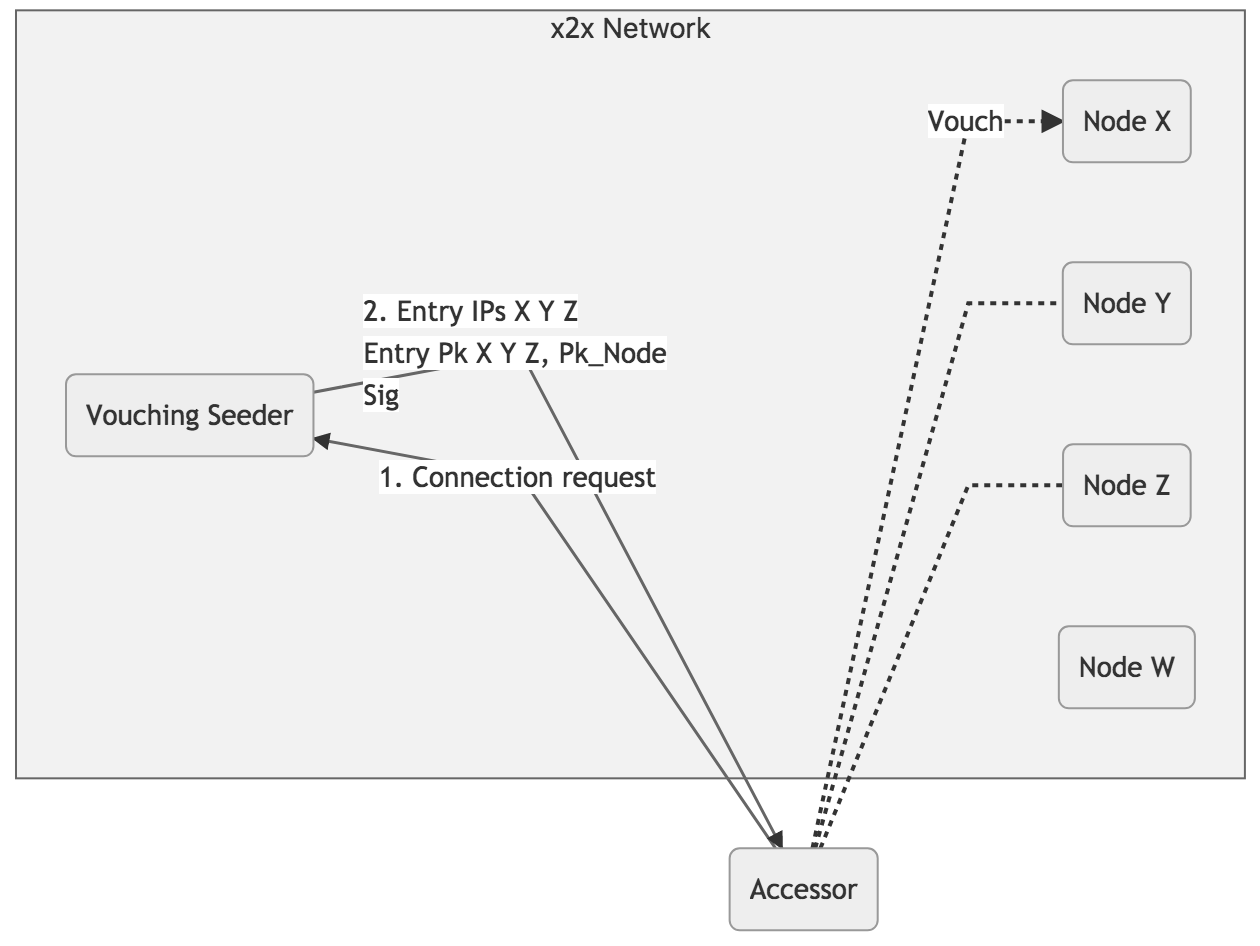
\includegraphics[scale=0.18]{bootstrap}
\caption{$x2x$ Network Bootstrap}
\label{boot}
\end{figure}

\begin{figure*}
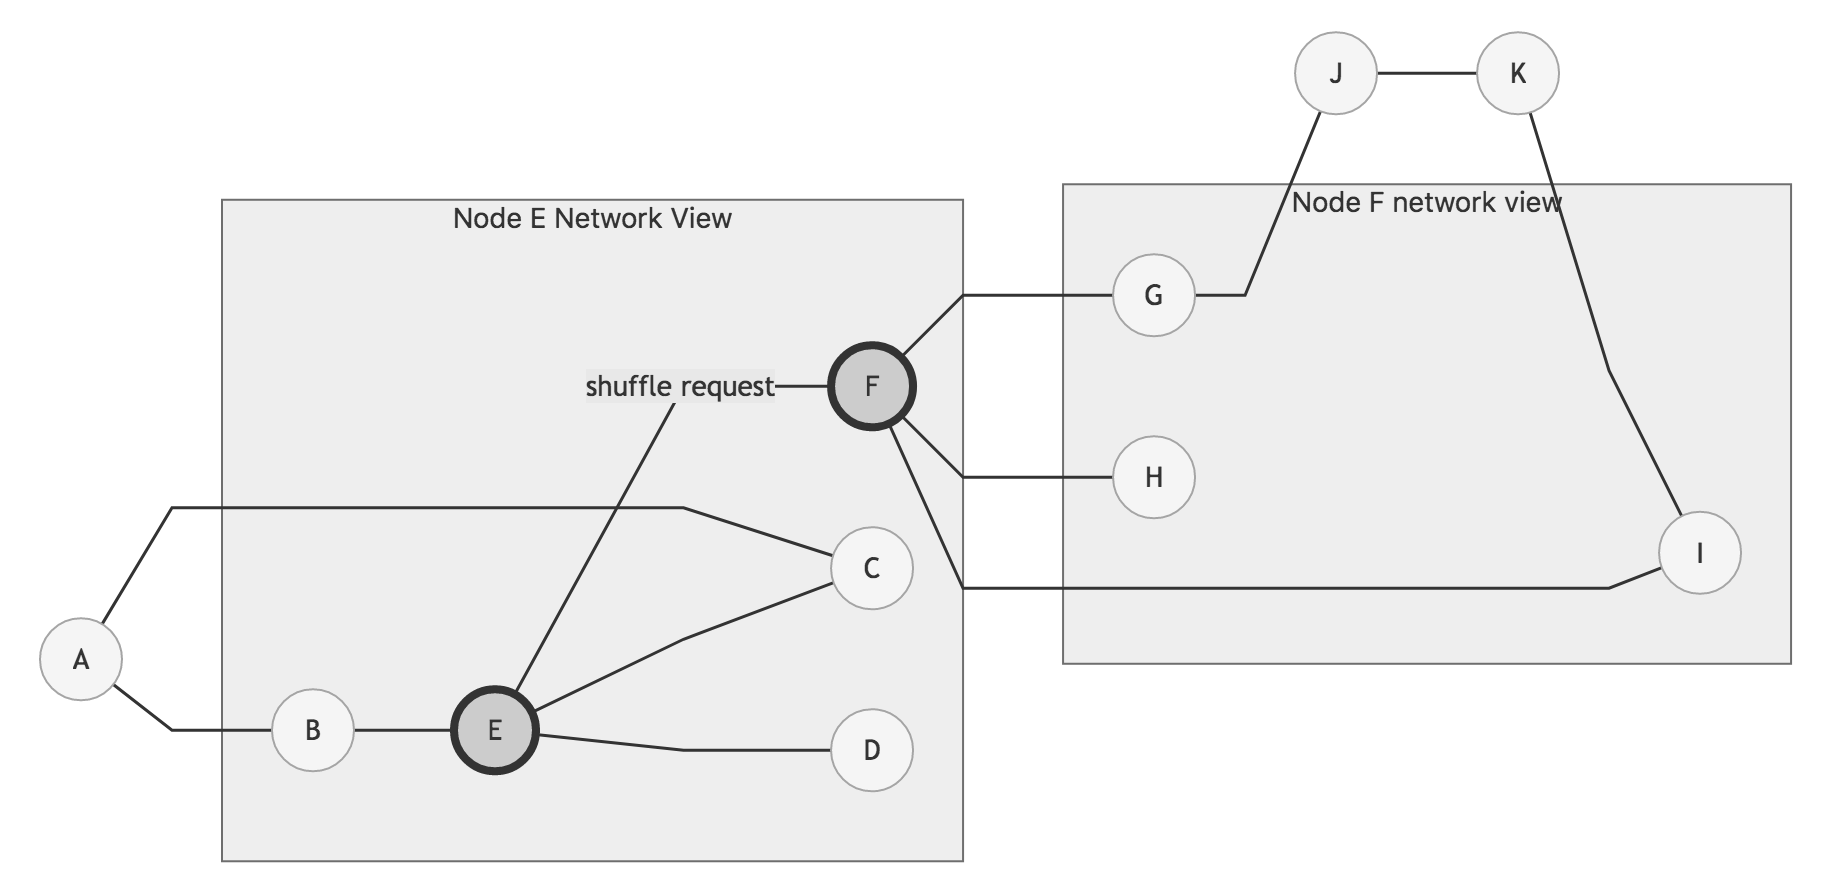
\includegraphics[scale=0.25]{gossip1}
\caption{Example gossip setup}
\label{goss1}
\end{figure*}


The accessor node thus selects an arbitrary end point \(X\) chosen among
those offered by the \emph{vouching seeder}. Thus, the accessor requests
\emph{Entry Tunnel} forming with \(X\) by sending the \emph{vouch} so
that \(X\) can verify the \emph{vouching seeder}'s signature and the
public key of the accessor, thus preventing potential IP routing leaks.
If the verification fails, the node refuses access, marks the node as
malicious and puts its IP into a distributed blacklist.

The accessor will then receive a set of active endpoints where
connection can be initiated, and will be assigned a hash which will act
as a mask for his real IP address. Similarly, the other nodes in the
network will be reachable solely through their own hash-mask. The
vouching seeders are trusted servers, reachable via a secured
\emph{https url} encoded into the \(x2x\) main core.

\subsection{Gossip Communication}



Once connected to the arbitrarily selected \emph{Entry Node},
\emph{Accessor} will become a full fledged member of the \(x2x\)
Network, and will receive from the \emph{Vouching Seeder} and the
\emph{Entry Node} an initial snapshot of \emph{\(x2x\) addresses} it can
gossip to. This internal, partial view of the network is constantly
maintained and refreshed by using a \emph{peer-sampling service}, which
is itself gossip-based. By using this service, the node will
periodically ask other nodes for an updated view of the network, and
will receive in return a set of addresses to update its internal view
with. For an efficient message spreading, it is also imperative that the
internal view of each node is as randomic as possible, and for this
reason the \emph{peer-sampling service} is also designed to maintain
high entropy within the network by occasionally shuffling nodes between
requesting peers.

Let's assume the structure in Figure \ref{goss1}, with nodes \(E\) and \(F\)
being two nodes about to shuffle addresses between each other.

In the scenario above, Node \(E\)'s internal node tables is
\([C, D, B, F]\) - which is the list of node addresses he knows about.
Node \(F\)'s internal node table will be instead \([G, I, H, E]\). When
shuffling nodes, the top of the head of each table is exchanged between
peers, so Node \(E\) will send to Node \(F\) the addresses \([C,B]\) and
in return will receive \([G,I]\). The new internal tables will modify
the network structure as in Figure \ref{goss2}.

\begin{figure*}
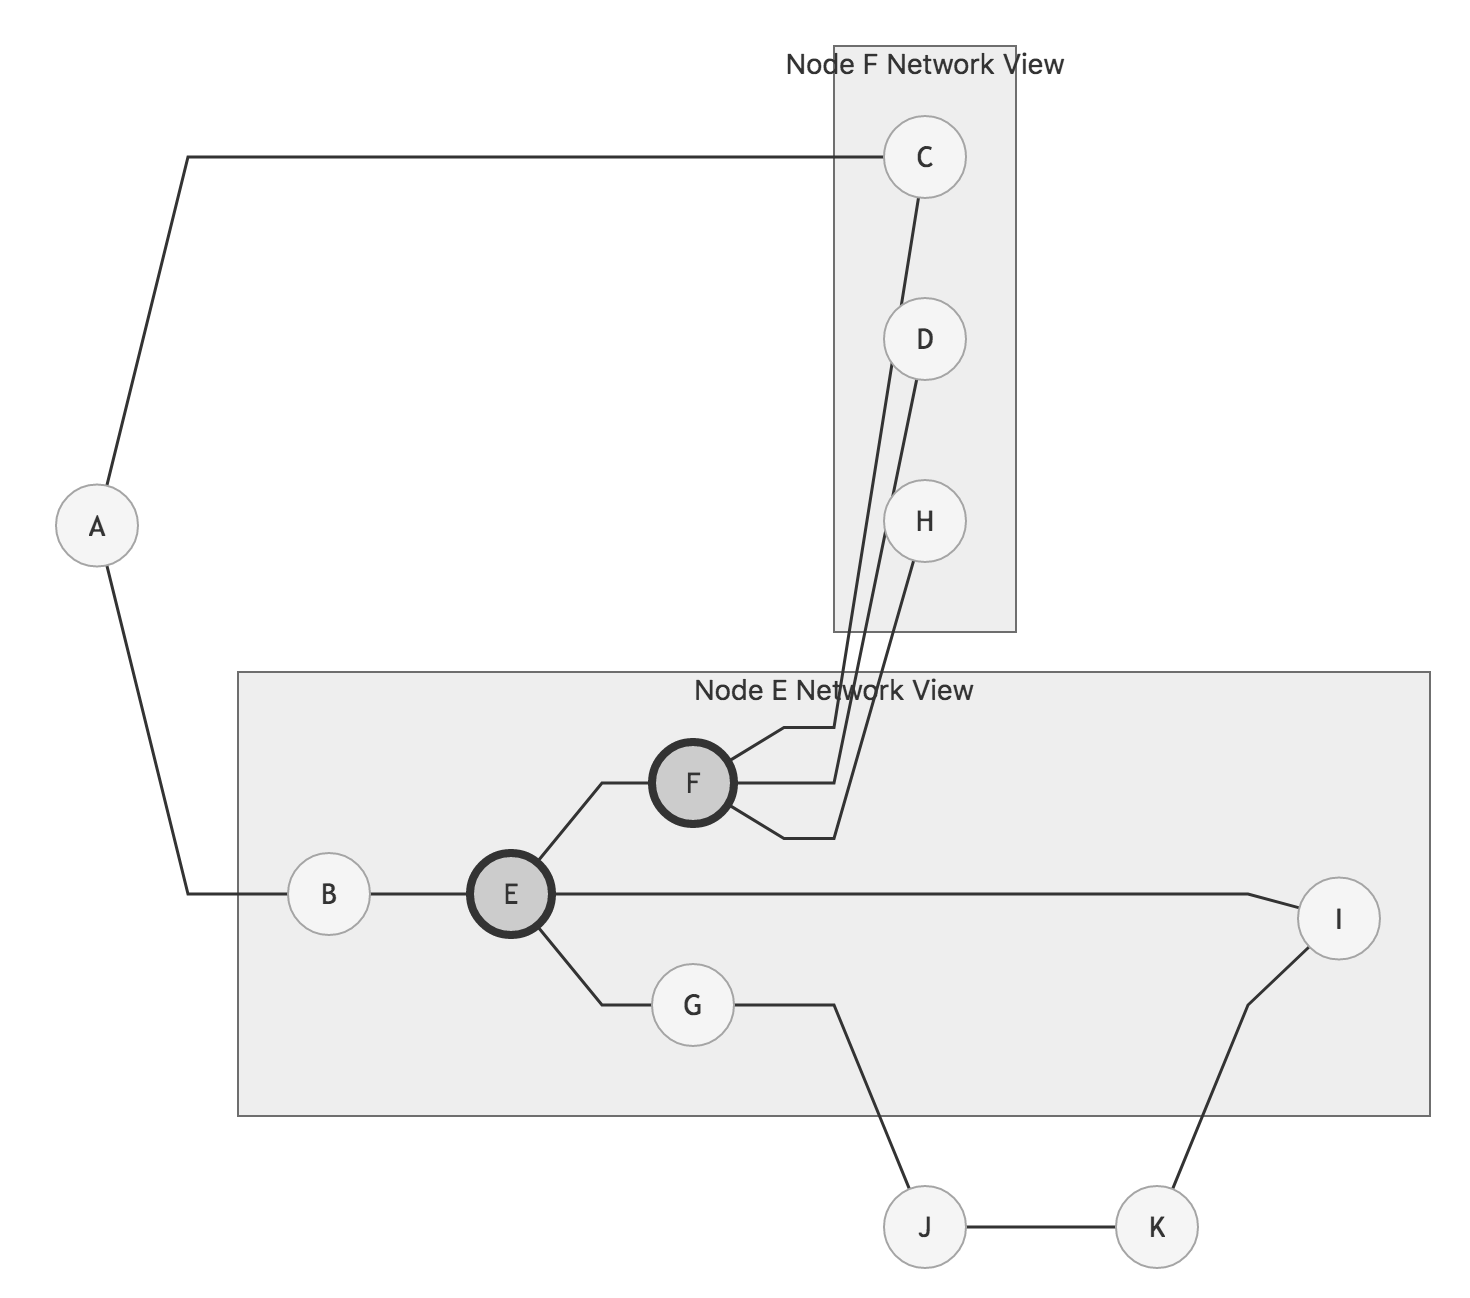
\includegraphics[scale=0.25]{gossip2}
\caption{Gossip setup post-shuffle}
\label{goss2}
\end{figure*}


This procedure ensures that configurations are never stagnant, and high
levels of randomness are always kept within the Network.


\subsection{Peer-Status Propagation}

Synchronising information about peer's \(x2x\) addresses happens with a
gossip-based communication scheme, called Peer-Status Propagation, which
is slightly more involved than the one used for transaction propagation
(which resembles more a \emph{fire-and-forget} approach). Peer-Status
Propagation shows resemblance to a TCP three-way handshake and it is a
suitable scheme to synchronise information relating to peer-sampling
table, a list of recent Provisioners, new peers joining the network or
addresses consistently in timeout. Another possibility (not explored in
this paper) is to exchange information about responsiveness of different
peers in order to stipulate a constantly updated overview of convenient
low-latency routes.

\begin{figure}
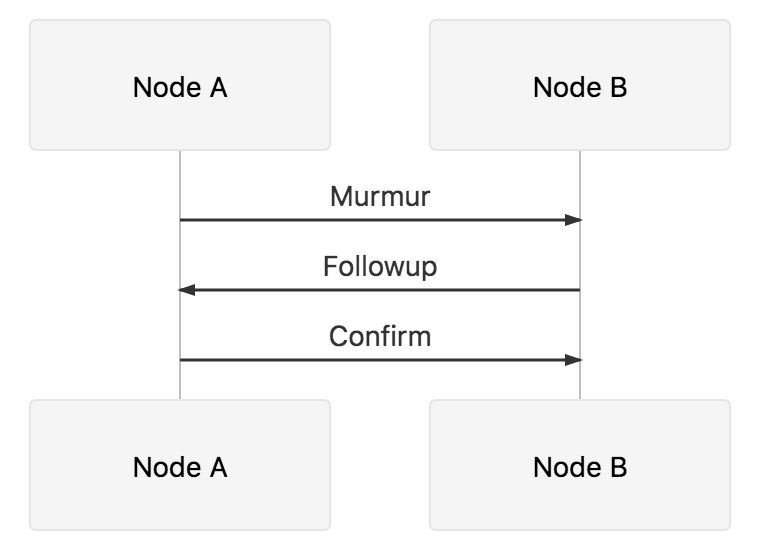
\includegraphics[scale=0.25]{peerprop}
\caption{Peer Status Propagation}
\label{peerprop}
\end{figure}

The information is exchanged as follows:

\textbf{Murmur} : The node initiating the communication sends out a
message to a receiving peer which contains his current view of the
network, plus information of the node itself (uptime, version), and
meta-data describing part of its internal status which he wishes to
transmit.

\textbf{Followup} : the receiving peer computes a difference between his
own meta-data and the one that was sent to it by the initiator. It then
follows up on the communication with a reply containing the gossip the
initiator ignores and a list of peer addresses the initiator does not
know about.

\textbf{Confirm}: After receiving the \emph{Followup} message, the
Initiator updates his meta-data with the message it just received by the
peer, saves the information, and sends out a \emph{Confirm} message with
the missing information the peer did not know about, if necessary. This
marks the end of the Status Propagation Round.

The increase of network traffic due to the Peer-Status Propagation is
constant and not expected to perceivably impact the efficiency of the
network. Relaying the \textbf{murmuring} is in fact limited to a
restricted amount of peers (i.e. three/four nodes) and \emph{Stata}
synchronization happens through the constant 2-phases Followup and
Confirm messages without causing any network spike.
\begin{figure*}
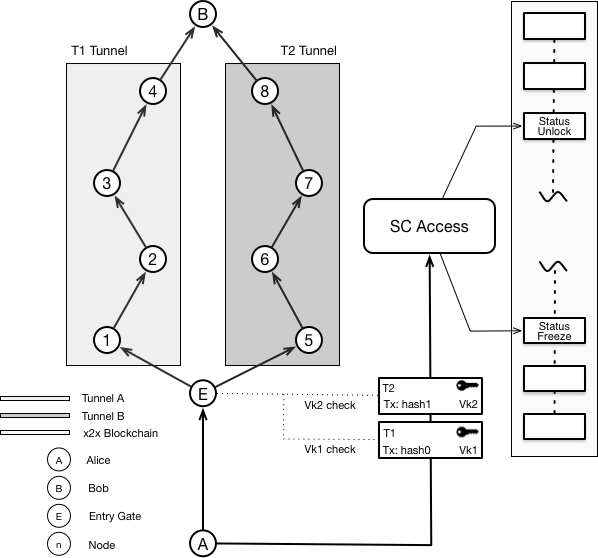
\includegraphics[scale=0.5]{tunnelswitch}
\caption{Tunnel Switching}
\label{tunnelswitch}
\end{figure*}
\subsection{Transaction Propagation}

The \(x2x\) blockchain makes use of advanced gossip network technology
in order to propagate transactions and sortition results for Block
Generator/Validators. Gossip protocols follow the \emph{endemic} message
dissemination system and represent a natural fit for a p2p network in
need to frequently synchronize small status variations among its peers
through the following advantages:

\begin{itemize}
\item
  \textbf{Scalability}: The general complexity of
  \href{https://pdfs.semanticscholar.org/3df0/523ff58d8dec53e89a521831265af32f52d6.pdf}{network
  gossip protocols}, is
  \href{https://arxiv.org/pdf/1512.03022.pdf}{\(O(logN)\)} which
  represents the number of rounds to reach all nodes in the network,
  where \(N\) is the total number of nodes. Nodes only send a limited
  number of messages and do not wait for acknowledgements. Such system
  can easily scale although it cannot achieve unbound scalability given
  the requirement of achieving global dissemination. In the case of
  \(x2x\) Blockchain, there is an inherent partition of nodes given by
  the fact that messages around block proposals, validations and voting
  is performed solely by Provisioners which relay these messages solely
  to other Provisioners.
\item
  \textbf{Error Tolerant}: \(x2x\) can operate extremely well with
  unreliable connections and unhortodox configurations. The same packets
  are sent multiple times to different peers - this way, should an
  infrastructure problem arise between two points impeding their
  communication, they will both receive the same message from other
  nodes in the network.
\item
  \textbf{Decentralization Ready}: there is no central role for any of
  the nodes. Each node works as an independent agent, with
  pre-established rules about data transmission.
\end{itemize}



A desirable property the \(x2x\) gossip protocol is to obtain relatively
low complexity while guaranteeing safety. For this is the reason, nodes
in the network do not relay more than one message/transaction coming
from the same node per \(\langle step, round \rangle\) of
\emph{SBA}\(\large\star\).

When a node wants to transmit information (transactions, sortition
results, etc.) it selects \(n\) random nodes from the set of nodes it
knows about (through the \emph{peer sampling service}) and transmits
such information to them, who, in turn, relay it further. Information
gets periodically sent to \(N\) targets, where \(N\) is known as the
\emph{Fanout}.

With \(Fanout=1\), we will need \(O(log N)\) \emph{Cycles} (which is the
number of rouds to spread a rumor) for the information to reach all
nodes.

In order to safeguard the anonymity of the peers, most of the messages
are relayed through anonymous datagrams following the specification of
I2P's \href{https://geti2p.net/spec/datagrams}{Non-Repliable Datagram},
which are packets devoid of sender \texttt{IP} information using the
\texttt{UDP} protocol. In the first instance of the \(x2x\) network, we
will make use of \href{https://geti2p.net/el/docs/api/samv3}{SAM v3}
protocol before considering rolling out a custom-made solution (which
might be necessary in case \(x2x\) will need to relay packets bigger
than 32Kb).




\section{Secure Tunnel Switching (STS)}

Powered by the \(x2x\) Blockchain, the \(x2x\) Network layer aims to
provide a next-generation, cryptographically secure way to perform
secure audio, video and data streaming between two distinct nodes on the
network. Current technologies limit themselves to establish a secure
connection between peers - but the \(x2x\) approach we are about to
describe goes far beyond that, by making sure that even if a node of the
network becomes compromised, the overall security of the platform as a
whole remains untouched.

\subsection{Setup}

We assume that node \emph{A} (Alice) wants to establish a secure data
stream connection with node \emph{B} (Bob), for which it knows the
relevant \(x2x\) address. Before initiating any connection attempt, node
\emph{A} will commit a payment towards a \emph{Smart Contract Access
Point (SCAP)} at instant \(T_1\), using an off-chain transaction, for a
dynamic value that will be auto-regulated by the \(x2x\) core. This is
done to keep the transmission cost stable, and also independent from
token fluctuations.

By receiving the transaction request, the \emph{SCAP} will freeze the
status on a block on the \(x2x\) chain for node \emph{A} - to be updated
later when the off chain transactions will come to an end.

Upon finalizing the transaction, node \emph{A} will contact her entry
point \emph{E}, and provide it with the \emph{view key} as proof of
payment. In turn, \emph{E} will check the validity of the key, and if
correct will allow the opening of a \emph{garlic routing tunnel} for a
duration of time \(\Delta_T\) towards node \emph{B}, so that node
\emph{A} can initiate the transmission.

At instant \(\Delta_T + \frac{\Delta_T}{2}\), node \emph{A} will start a
new transaction with \emph{SCAS} to renew the duration of such tunnel
for an additional interval \(\Delta_T\), and if successful will open a
new tunnel with \emph{B}, and will start sending a concurrent, identical
data stream on the new one. Node \emph{B} will consequentially drop the
previous tunnel using a procedure that we will describe below. This
process we illustrate will continue until the data transmission will
come to an end, by either \emph{A} choosing to not renovate a tunnel or
failing to complete a new transaction with the \emph{SCAP}.

If node \emph{A} does not provide her Entry point \emph{E} with a valid
view key for the next transaction, the tunnel will be dropped entirely
from the Entry point itself.

\subsection{Tunnel Switching}

Once received the data stream from sender node \emph{A}, receiver node
\emph{B} will parse the raw data (which can be a VoIP call, for example)
and will keep waiting for new tunnel connections. Upon receiving a
second connection, \emph{B} will match the two data stream by doing a
trivial bit matching operation, which will almost certainly show a small
time lag due to the fact that the two tunnels use a different set of
relaying nodes. (Figure \ref{datamatch})

\begin{figure}
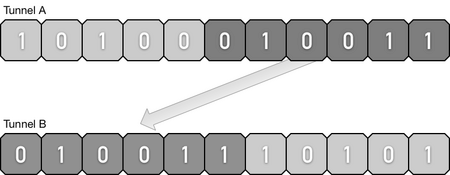
\includegraphics[scale=0.5]{dataswitch}
\caption{Data Match + Switch}
\label{datamatch}
\end{figure}

After successfully matching the streams, node \emph{B} can safely
discard the old one, and continue parsing the stream on the most recent
one. The procedure will repeat for as long as sender node \emph{A} will
renew the transaction costs with the \emph{SCAS} to keep streaming data.


The following approach dramatically improves security and anonimity over
a conventional \emph{Garlic Tunnel} connection. By switching the data
tunnel at regular intervals, a malicious attacker would be unable to
predict compromised nodes, perform DDoS attacks, and in general exploit
vulnerabilities on the network.

\section{On- Offline File Transfer}

The capability to anonymously and securely send files over the network
and allow both offline and online retrieval is a unique feature of the
\(x2x\) Network. To implement such a use-case, \(x2x\) combines the
capabilities of the anonymous peer discovery and gossip mechanism
previously described with those of the \href{https://orc.network/}{Orc
Object Storage}, a third party decentralised and anonymous storage
service. The workflow to securely send a file over the network is the
following:

- Alice encrypts file.doc using \(\textrm{camellia-256}\) using Bob's
\(P_k\) - Alice will upload the file to the Orc Cloud Network, and will
get the \texttt{id} of the file once the upload is complete - Alice will
create an Anonymous Non-Repliable Datagram with the following structure:

\begin{center}\rule{0.5\linewidth}{\linethickness}\end{center}

\texttt{1:\ T7CvGQr0/nq8xiLfekdTUGz6rQggGnYYOxuXrMf4vPw=}\\
\texttt{2:\ GT7RzkvXJIPjT0xpJXVIhu6QjIzElxKDuvcJKyguwK3HT6GZaRA\\9/O4+XCKF67wNeyTfn8RGPM53lp0z+MLW2w==}

\begin{center}\rule{0.5\linewidth}{\linethickness}\end{center}

\begin{figure}
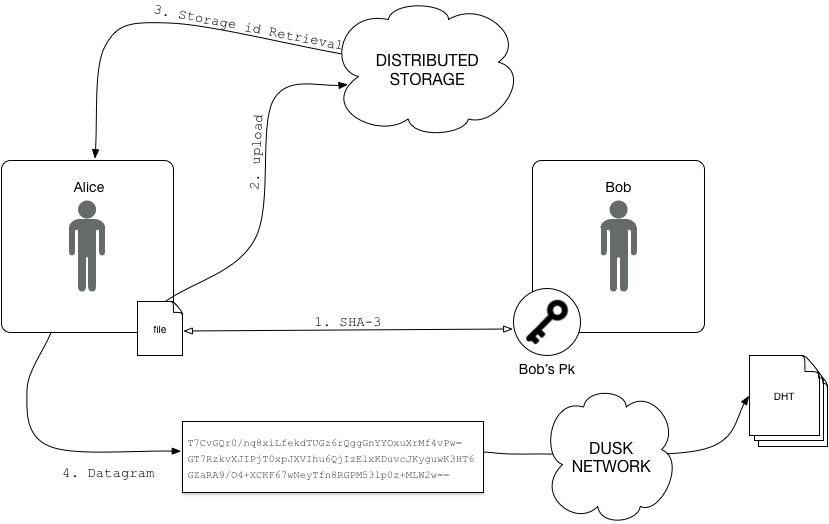
\includegraphics[scale=0.20]{orc}
\caption{Secure File Transfer}
\label{orc}
\end{figure}

The first line of the datagram is the \(\textrm{camellia-128}\)
encrypted \texttt{id} of the file on the Orc Network (using Bob's
\(p_k\)) and will be used to retrieve such file. Second line is Bob's
\(x2x\) Address, also encrypted with \(\textrm{camellia-128}\) using
bob's \(p_k\). In case Alice would like Bob to know she was the sender
of the file, she will add a third line with her own x2x address, also
encrypted with \(\text{camellia-128}\) using Bob's \(p_k\).

We will now have two separate cases, since Bob can be online when the
file is sent, or offline.

\begin{itemize}
\item
  Bob is \textbf{online} --- Bob receives Alice's datagram, checks if he
  is the owner of the file by trying to decrypt the second line with his
  private key \(s_k\). If successful will also decrypt the first line
  and download the file from Orc.
\item
  Bob is \textbf{offline} --- The entry will be inserted in a
  distributed hash table (DHT) and kept there for 30 days, which Bob can
  interrogate as soon as he is online in order to check for files that
  were addressed to him while he was away. The DHT will be supported by
  extending the \emph{Provisioner} protocol with a simplified version of
  the RPC primitives of
  \href{http://xlattice.sourceforge.net/components/protocol/kademlia/specs.html\#protocol}{Kademlia
  Specifications} implemented over Non-Repliable Datagrams.
\end{itemize}


\section{Conclusions}

$x2x$ Network is an unrestricted, unsurveilled and fully distributed cryptosystem designed for high-rate voice and data communications, enforcing the utmost level of privacy to the partaking peers. The network features a novel blockchain-based digital cash called $x2x$, used to directly incentivize participation in the network and promote widespread adoption. $x2x$ features untraceability through the use of ring confidential transactions, unlinkability through the use of stealth address and protection from sybil attack and double spending through a novel consensus algorithm called Segregated Byzantine Agreement or SBA$\large\star$. SBA$\large\star$ provides direct block finality by preventing forking while providing virtually unbounded scalability. The network is built on top of an efficient gossip network which utilizes non-repliable datagram and garlic routing in order to prevent IP Address propagation. Finally, the $x2x$ Network is complemented with an off- online file transfer mechanism and with realtime $x2x$ payment channel to enable undetectable and fast peer-to-peer data communication through a technique we call Secure Tunnel Switching.